% !TEX root = ../../Beamer/statikz/statikz.tex


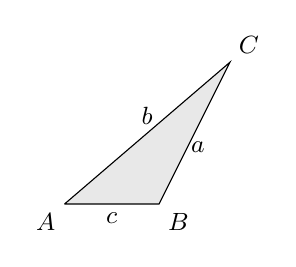
\begin{tikzpicture}[scale=0.6]

	\coordinate (A) at (0,0);
	\coordinate (B) at (2,0);
	\coordinate (C) at (3.5,3);

	\small
	\filldraw[fill=Gainsboro!65, draw=black] (A) -- node[below] {$c$}(B) --  node[below] { \;$a$}(C) --  node[above] {$b$} (A);

	\draw[below right] (B) node {$B$};
	\draw[below left] (A) node {$A$};
	\draw[above right] (C) node {$C$};
	
\end{tikzpicture}
